\subsection{Change}
\label{sec:Suggestion:Change}

\begin{figure}[t]
    \centering
    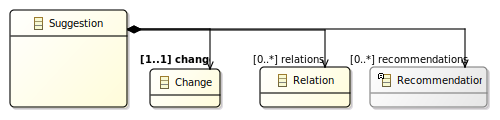
\includegraphics[width=\columnwidth]{images/Suggestion.pdf}
    \caption{A \textsf{Suggestion} holds for a single \textsf{Change} linked to 
		elements in a View Type through \textsf{Relation}s, and consists of a set of \textsf{Recommendation}s.}
    \label{fig:Suggestion}
\end{figure}

A \textsf{Change} refers to an \textsf{Operator} that may be parameterised with 
extra data, and contains contextual information (in \textsf{ApplicationPattern}). 
Change \textsf{Operator}s may target \emph{any} instanciable metamodel element, 
thus referring to the class \textsf{NamedElement} in \textsc{Mof}. Note that we 
will distinguish between \emph{primitive} and \emph{complex} \textsf{Operator}s,
depending on the number of such \metamodel elements an \textsf{Operator} acts on.

Since \viewtypes are structurally \metamodels, we reviewed the literature to
identify relevant change \textsf{Operator}s. The change catalogue proposed by 
\cite{herrmannsdoerfer_extensive_2011} presents 27 \emph{primitive}, and 34
\emph{complex} operators. We integrated all primitive, and 7 complex operators
in our work, which were selected because they constitute 72\% of all complex
changes appearing in a large case study (cf. \cite{khelladi_detecting_2015}). 

\textsf{Operator}s are enriched with a \emph{severity}: \emph{Major}
(abbreviated as \textsf{M}), \emph{miNor} (\textsf{N}) and \emph{Ignore} 
(\textsf{I}). 
When applied to a \metamodel, the \textsf{Operator}s in \textsf{I} have no effect
on the corresponding \viewtypes; \textsf{Operator}s that can break the relationship
between \textsf{MM }and its \viewtypes are categorised as \textsf{M}; the rest of the
\textsf{Operator}s are \textsf{N}, since they are not breaking and can enrich 
the \viewtypes with additional information.
\MA{Align MM in figures + Extend with op-relevant info}

\begin{figure}[t]
    \centering
    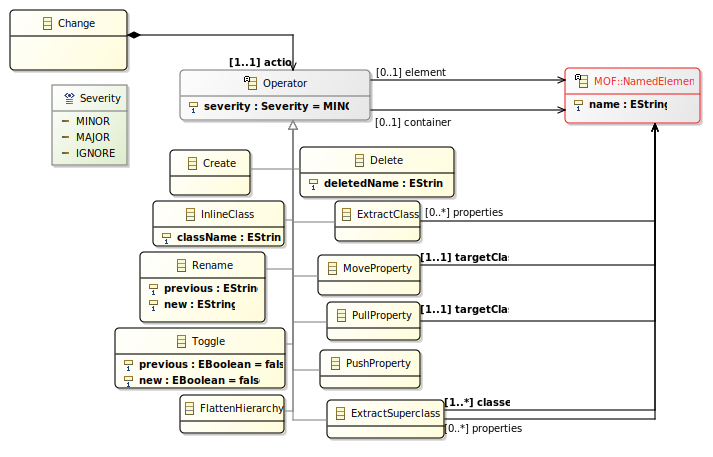
\includegraphics[width=\columnwidth]{Change.pdf}
    \caption{Possible \textsf{Change}s operated on a \metamodel.
		\MA{Note that the \textsf{NamedElement}s actually come from two different MMs!}}
    \label{fig:Change}
\end{figure}
